\documentclass[11pt,pdftex,portrait,letterpaper]{article}
\usepackage[hdivide={1in,*,1in},
vdivide={1in,*,1in},
%            showframe
]{geometry}

% Standard packages
\usepackage[T1]{fontenc}
\usepackage{graphicx}
\usepackage{longtable}
\usepackage{acronym}
\usepackage{verbatim}
\usepackage{subfigure}
\usepackage{fancyhdr}
\pagestyle{fancy}
\usepackage{listings}
\usepackage{color}
\usepackage{lastpage}
\usepackage{caption}

% Fonts
%\usepackage{libertine}	% Libertine (the main font)
%\usepackage[lcgreekalpha]{libertinust1math}	% Libertine (as the math font)
\usepackage[varl]{inconsolata}	% A monospace font similar to Consolas. The varl option makes the lowercase l look different than a numeral 1.

% Last packages
\usepackage[hidelinks]{hyperref}	% Hyperlinks

% Modify parameters of Listings
\definecolor{lstgreen}{rgb}{0,0.6,0}
\definecolor{lstgray}{rgb}{0.4,0.4,0.4}
\lstset{ 
	language=C,
	basicstyle=\ttfamily\scriptsize,
	numbers=left,
	numberstyle=\footnotesize,
	keywordstyle=\color{blue},
	identifierstyle=\color{black},
	commentstyle=\color{lstgreen},
	stringstyle=\color{lstgray},
	stepnumber=1,
	numbersep=10pt,
	backgroundcolor=\color{white},
	frame=single,
	captionpos=b,
	breaklines=true,
	breakatwhitespace=false,
	tabsize=2,
	showstringspaces=false
}

% Default margins are too wide all the way around. Reset them here
\setlength{\topmargin}{-.5in}
\setlength{\textheight}{9in}
\setlength{\oddsidemargin}{0in}
\setlength{\textwidth}{6.5in}

\lhead{ECEN 220}
\chead{ADC Project 2}
\rhead{\thepage\ of \pageref{LastPage}}
\lfoot{\small{University of Nebraska--Lincoln}}
\cfoot{}
\rfoot{\small{Department of Electrical \& Computer Engineering}}
\renewcommand{\footrulewidth}{0.5pt}




\begin{document}
	
	\vspace*{30ex}
	\begin{center}
		
		\textbf{ADC Project 2}\\
		
		\vspace{4ex}
		ECEN 220: Introduction to Embedded Systems\\
		University of Nebraska--Lincoln\\
		March 6, 2021
		
		\vspace{4ex}
		Name: David Perez\\
		
	\end{center}
	
	
	\pagebreak
	\tableofcontents
	%\pagebreak
	%\listoffigures
	%\addcontentsline{toc}{section}{{\bf List of Figures}}
	\pagebreak
	
	
	\section{Introduction}

	During this project, the intention was to delve inside our ATmega329P and gain an understanding of the ADC registers. An ADC is simply and analog to digital converter. This allows us to read real world signals such as the the voltage of a circuit by converting our ADC values into a voltage value. In this project this is achieved by multiplying the value in the ADC register and multiplying it by (5.0 / 1024).  This multiplier is derived from the fact that we set our reference voltage to 5v in our ADMUX register and in our ADC register consits of 10 bits (2$^{10}$ = 1024).
	
	In the first program of this project we used 5v as our reference but, the second program sets the reference voltage to 1.1v. As you'll soon find out, the ADC isn't entirely accurate so by changing the reference we can increase the accuracy of our ADC. This is straight forward due to the fact that 1.1 / 1024 = 0.00107 while 5/1024 = 0.00488 which in our case is equivalent to 1.04mv to 4.88mv meaning we can increase the accuracy by almost 4 fold.
	
	
		\section{Program Description}
	

	
	Behind each program in this project there is an important underlying on why we created each one. For our first program our task was to see see how the adc actually operates and record our results. This was accomplished by setting our reference voltage  to 5v in the ADMUX register.Using a potentiometer and our Arduino nanos 5v we adjusted the input voltage to our ADC from 0 to 5v. We then began the conversions using the ADCSRA	register. After the conversion was complete, we retrieved the value in the ADC register and multiplied the 10bit value by 5.0 /1014. This converted value would give us our ADC's estimated voltage which we would then compare with the voltage that we would measure using a digital multimeter.
	
	We performed a similar experiment to program 1 with program 2. The difference here was that we differed our reference voltage from 5v to 1.1v. With this we tested ranges from 0 to 1.1v and compared our adc value with the measured value from our digital multimeter. On top of this, we would also derive an expected ADC value to compared with our recorded one and place all these values in a table (The tables for each program and the correspoding values are displayed below).
	
	As for program 3, our goal was to time the duration of an ADC conversion. Using information from the first project we were tasked to enable the PB0 as an input pin. Once we initialize the pin high, we would begin and ADC conversion and once it was completed turn the PB0 pin low. With this we were able to calculate the actual time it took for a conversion to complete and compare that result with that of the 13 cycles claimed on the ATmega329P data sheet	
	\subsection{Program 1}
	 
	When executing this program and performing this experiment there were a couple of things to keep in mind. The first of which is pretty obvious but the ADC doesn't allow a voltage below 0 meaning it can't contain a negative value. On the other side of the coin, the ADC doen't actually allow for measuring 5v. This is due to the ammount of error the ADC has in the sense that when applying 4.75v (the max voltage possible from the Arduinos 5v output) the ADC outputs a value of 1023 which is the max value the ADC can contain. 
	
	In the table below it may initially seem strange as to why the expected ADC value and the recorded ADC value aren't the same. There are many factors that this can result from but for now I'm going to just list a few. The first of which is simply just digital error, meaning that like all digital and electrical things there is noise and marginal error that come out. This is especially evident and more widely producted products and cheaper electronics that aren't entirely accurate in filtering out this noise. Another thing would be how the conversions actually take place. The ADC register cannot hold a value that is a decimal value so when it it doing the conversion by multiplying the input voltage by 1024, and dividing it by 5 it is guranateed that there is a chance of it being off by around 4.48mv due to it rounding up or down.
	
\begin{table}[htb]
	\centering
	\begin{tabular}{ | c | c | c | c | }	% add more columns (r, c, or l for the justification) and column separators (|) here
		\hline
		\textbf{Measured v$_{in}$} & \textbf{Expected ADC Value} & \textbf{Recorded ADC Value} & \textbf{Converted ADC Voltage} \\ \hline \hline
		0.00v & 0 & 0  & 0.00v \\ \hline
		0.30v & 61.44 & 64  & 0.31v \\ \hline
		0.67v & 137.22 & 144  & 0.70v \\ \hline
		1.22v & 249.86 & 262 & 1.28v \\ \hline
		2.03v & 415.74 &  437 & 2.13v \\ \hline
		2.33v & 477.18 &  503 & 2.46v \\ \hline
		2.92v & 598.02 &  629 & 3.07v \\ \hline
		3.95v & 811.01 &  852 & 4.16v \\ \hline
		4.46v & 913.41 & 961  & 4.69v \\ \hline
		4.75v & 972.8 & 1023  & 5.00v \\ \hline
		
	\end{tabular}
	\caption{Program 1 Results with "v" representing volts }
	\label{t:table1}	% labels must come after the caption
\end{table}
	
	
	
	\subsection{Program 2}
	
Program 2 differs from the fist by a few things but most importantly being the change in reference voltage. Doing this allowed us to increase the accuracy of our ADC but results in having a smaller range of voltages we can measure. Again we could only measure down to 0v but can only meausure up to give or take 1.1v. Because of the increased accuracy by having each bit of the ADC correspond to about 1mv 4s 4.48mv using the 5v reference our expected adc value was significanly closer to the recorded ADC value. This is evident if you examine the table from program 1 versus that of program 2. 

These measurements were a lot closer to my expectations but it still came as a suprise off the ADC could actually be. When increasing the voltages in both programs would become increasingly inaccurate which most likely results in the 5 \% that tends to result when performing electrical experiments among the many other factors listed in program 1.
	
	
\begin{table}[htb]
	\centering
	\begin{tabular}{ | c | c | c | c | }	% add more columns (r, c, or l for the justification) and column separators (|) here
		\hline
		\textbf{Measured v$_{in}$} & \textbf{Expected ADC Value} & \textbf{Recorded ADC Value} & \textbf{Converted ADC Voltage} \\ \hline \hline
		0.00v & 0 & 0  & 0.00v \\ \hline
		0.05v & 46.55 & 45  & 0.05v \\ \hline
		0.10v & 93.01 & 96  & 0.10v \\ \hline
		0.18v & 167.56 & 166 & 0.18v \\ \hline
		0.25v & 232.73 &  241 & 0.26v \\ \hline
		0.34v & 316.52 &  317 & 0.34v \\ \hline
		0.54v & 502.69 &  510 & 0.55v \\ \hline
		0.75v & 598.18 &  710 & 0.76v \\ \hline
		0.98v & 912.29 & 929  & 1.00v \\ \hline
		1.10v & 1024 & 1023  & 1.1v \\ \hline
		
	\end{tabular}
	\caption{Program 2 Results with "v" representing volts }
	\label{t:table1}	% labels must come after the caption
\end{table}

	\pagebreak
	
	\subsection{Program 3}
	
For program 3 our objective was to see how long the it actually took for the ADC to make a conversion. This was accomplished by setting PB0 high then starting the conversion, then once complete setting PB0 low. Using the logic analyzer this enabled us to find the time it took to make the conversion.

From the figure below, the actual measured time was about 111.7 microseconds. My predicted conversion time was 104 miscroseconds which was derived by taking 1 / 125kz to get the ADC clock rate and then multiplying it by the 13 clock cycles it takes according to the datasheet. Taking into consideration the ammount of time it takes to set PB0 high and low as well as the jmp function that restarts, I'd consider this to be a pretty accurate conversion time.  Another takeaway form this program was the maximum sample rate that our ADC can handle. This values come our to 15000SPS which means that if we try to sample any faster than that it would result in garbage ADC values.

	\begin{figure}[h]
		\centering
		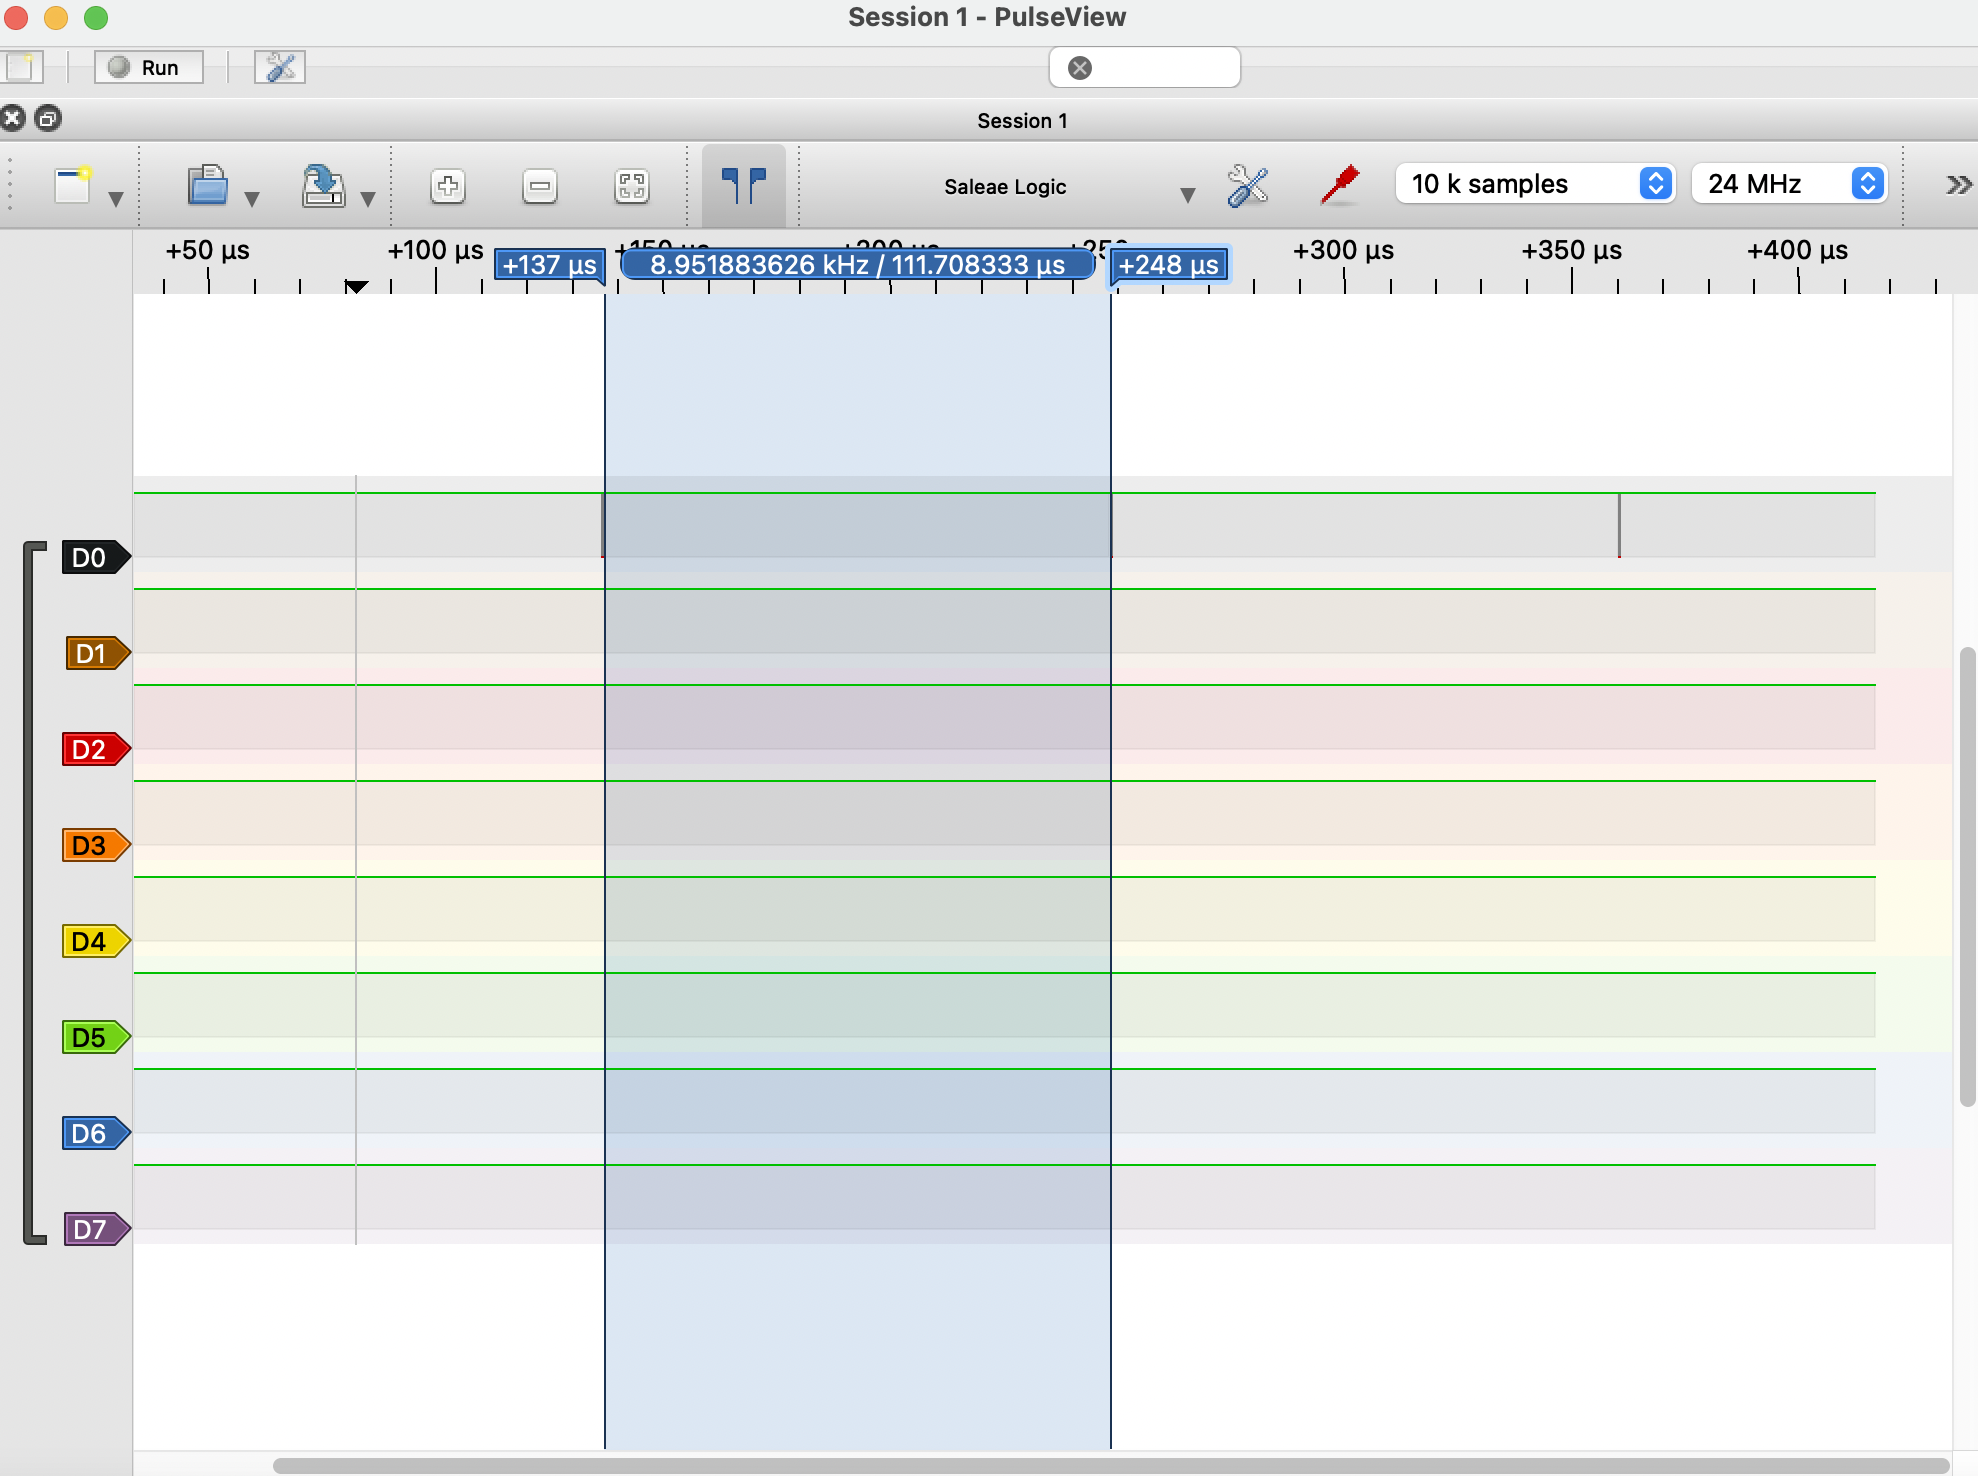
\includegraphics[width=0.9\textwidth]{./program3_conversionTime}	% The .png file will be used to make the figure here, and is in the same directory as this .tex file
		\caption{Screen Capture of program 3 ADC Conversion Time}
		\label{f:fig1}	% labels must come after the caption
	\end{figure}
	\pagebreak
	
	
	\section{Conclusion}
	
Every program in this project contributed to some very important information about how the ADC works on the Arduino nano MCU. In programs 1 and 2 we initialized some of the fundamental abilities of the ADC. With program 1 we set the reference voltage to 5v which allowed for a 4.88mv assignment for each bit of the ADC registers. When changing the reference voltage to 1.1v like in program 2 we increased our accuracy by almost 4 fold. This concluded in our measurements to be significanlty more accurate when measuring voltages between 0-1.1v than that of 0-5v. Regardless though, there was still some error when measuring the voltages using the ADC and this was evident what measuring the actual voltage using a multimeter and comparing the values. From program 3 we saw the conversion time of the ADC and compared that value with the theoretical value. Again these values were close but not entirely the same due to many factors such as the time delays from the other instructions in our program. In conclusion, we were able to understand how to use the ADC registers and how they could be used to read voltages.
	
	\pagebreak
	
	\section{Appendix}
	
	%Here is an example of how to add good-looking code snippets using a 'listing' 
	\begin{lstlisting}[caption={Program 1}, label=l:programx]
	/** Includes **/
	#include <stdint.h>
	#include <Arduino.h>
	#include <stdio.h>
	
	
	/** memory mapped registers also our global variables **/
	volatile uint8_t* ioADMUX;  //adc multiplexer selection register
	volatile uint8_t* ioADCSRA; // control and status registers
	volatile uint8_t* ioADCL;   // adc low conversion bits
	volatile uint8_t* ioADCH;   //adc high conversion bits
	
	/** Main function **/
	int main(void){
		
		//Initialize the Arduino Wiring Library
		init();
		
		//Set up our serial port at 9600 bps (baud rate)
		Serial.begin(9600);
		
		//Populate the MMR pointers with the adresses
		ioADMUX = (volatile uint8_t) 0x7C;
		ioADCSRA= (volatile uint8_t) 0x7A;
		ioADCL = (volatile uint8_t) 0x78;
		ioADCH = (volatile uint8_t) 0x79;
		
		/*First, configure the ADMUX register */
		//REFS[1:0] = 0b01 for AVCC (0b11 for 1.1v reference)
		// bit 4 of mux == 0b0
		//ADLAR(bit 5) = 0b0 to be "right adjusted"
		//MUX[3:0] = 0b0010 to select ADC2 which is pin A2 on arduino or PC2
		// concat and place in ioADMUX == 0b01000010
		*ioADMUX = 0x42;
		
		/* Next, configure the ADCSRA register */
		//ADEN = 0b1 to enable ADC
		//ADSC = 0b0 so that that we don't start conversion early
		//bits 5 4 3 we ignore and set to 0's
		// ADPS[2:0] = 0b111 to selecte the prescalar division ratio as 128
		// so that (16Mhz / 128 = 125Khz, which is in between 50 and 200khz as per spec
		//concat and place in ioADCSRA == 0b10000111 = 0x87
		*ioADCSRA = 0x87;
		
		//Do an infinite loop that continously prints the ADC value after it finished converting
		while(1)
		{
			//Start the ADC conversion
			//To do this, we need to set ADSC (thich is the bit 6 of the
			//ADCSRA register) to a 0b1
			//Read-write-modify
			//  *ioADCSRA = (*ioADCSRA) | 0x40;   //0b01000000
			*ioADCSRA |= 0x40;  // same as line above
			
			/* wait for ADC to finish converting */
			
			while(((*ioADCSRA) & 0x40) != 0x00)
			{
				// loop untils bit 6 of ADCSRA is 0 
				// indicating a completed conversion
			}
			
			/* ADC conversion is complete */
			//read ADCL value first
			uint8_t adc_low_value = *ioADCL;
			
			//Now, read the ADCH register
			uint8_t adc_high_value = *ioADCH;
			// combine into a 16 bit integer
			uint16_t adcResult = adc_low_value & 0x00FF;
			//convert high value to 16 bits and left shift 8 bits
			adcResult = (adcResult) | ((uint16_t)adc_high_value << 8);
			
			
			//print out the ADC output code
			char message[80];
			sprintf(message, "ADC output code: %u \n", adcResult);
			Serial.write(message);
			
			float AdcVoltage;
			
			//convert the ADC code to a estimated voltage
			AdcVoltage = (5.0 / 1024.0) * adcResult;
			Serial.write("ADC voltage is: ");
			Serial.print(AdcVoltage);
			Serial.write("v\n");
		}
	}
	
	\end{lstlisting}
	
	\begin{lstlisting}[caption={Program 2}, label=l:programx]
		
		/** Includes **/
		#include <stdint.h>
		#include <Arduino.h>
		#include <stdio.h>
		
		
		/** memory mapped registers also our global variables **/
		volatile uint8_t* ioADMUX;  //adc multiplexer selection register
		volatile uint8_t* ioADCSRA; // control and status registers
		volatile uint8_t* ioADCL;   // adc low conversion bits
		volatile uint8_t* ioADCH;   //adc high conversion bits
		
		/** Main function **/
		int main(void){
			
			//Initialize the Arduino Wiring Library
			init();
			
			//Set up our serial port at 9600 bps (baud rate)
			Serial.begin(9600);
			
			//Populate the MMR pointers with the adresses
			ioADMUX = (volatile uint8_t) 0x7C;
			ioADCSRA= (volatile uint8_t) 0x7A;
			ioADCL = (volatile uint8_t) 0x78;
			ioADCH = (volatile uint8_t) 0x79;
			
			/*First, configure the ADMUX register */
			//REFS[1:0] = 0b11 for internal 1.1v reference
			// bit 4 of mux == 0b0
			//ADLAR(bit 5) = 0b0 to be "right adjusted"
			//MUX[3:0] = 0b0101 to select ADC5 which is pin A5 on arduino or PC5
			// concat and place in ioADMUX == 0b11000101
			*ioADMUX = 0xC5;
			
			/* Next, configure the ADCSRA register */
			//ADEN = 0b1 to enable ADC
			//ADSC = 0b0 so that that we don't start conversion early
			//bits 5 4 3 we ignore and set to 0's
			// ADPS[2:0] = 0b111 to select the prescalar division ratio as 128
			// so that (16Mhz / 128 = 125Khz, which is in between 50 and 200khz as per spec
			//concat and place in ioADCSRA == 0b10000111 = 0x87
			*ioADCSRA = 0x87;
			
			//Do an infinite loop that continously prints the ADC value after it finished converting
			while(1)
			{
				//Start the ADC conversion
				//To do this, we need to set ADSC (thich is the bit 6 of the
				//ADCSRA register) to a 0b1
				//Read-write-modify
				//  *ioADCSRA = (*ioADCSRA) | 0x40;   //0b01000000
				*ioADCSRA |= 0x40;  // same as line above
				
				/* wait for ADC to finish converting */
				
				while(((*ioADCSRA) & 0x40) != 0x00)
				{
					// loop untils bit 6 of ADCSRA is 0 
					// indicating a completed conversion
				}
				
				/* ADC conversion is complete */
				//read ADCL value first
				uint8_t adc_low_value = *ioADCL;
				
				//Now, read the ADCH register
				uint8_t adc_high_value = *ioADCH;
				// combine into a 16 bit integer
				uint16_t adcResult = adc_low_value & 0x00FF;
				//convert high value to 16 bits and left shift 8 bits
				adcResult = (adcResult) | ((uint16_t)adc_high_value << 8);
				
				//print out the ADC output code
				char message[80];
				sprintf(message, "ADC output code: %u \n", adcResult);
				Serial.write(message);
				
				float AdcVoltage;
				
				//convert the ADC code to a estimated voltage
				AdcVoltage = (1.1 / 1024.0) * adcResult;
				Serial.write("ADC voltage is: ");
				Serial.print(AdcVoltage);
				Serial.write("v\n");
			}
		}
		
	\end{lstlisting}
	
		\begin{lstlisting}[caption={Program 3}, label=l:programx]
			/** Includes **/
			#include <stdint.h>
			#include <stdio.h>
			
			/** GLOBAL Variables */
			volatile uint8_t* pDDRB;
			volatile uint8_t* pPORTB;
			
			//global variables for ADC
			volatile uint8_t* ioADMUX;  //adc multiplexer selection register
			volatile uint8_t* ioADCSRA; // control and status registers
			volatile uint8_t* ioADCL;   // adc low conversion bits
			volatile uint8_t* ioADCH;   //adc high conversion bits
			
			/* Main Function */
			int main(void)
			{
				// Define our pointers to the GPIO registers 
				pDDRB = 0x24;
				pPORTB = 0x25;
				
				// Set PB0 as an output with the DDRB register
				*pDDRB = 0x01; // 0x01 = 0b00000001
				
				//Populate the MMR pointers with the adresses
				ioADMUX = (volatile uint8_t) 0x7C;
				ioADCSRA= (volatile uint8_t) 0x7A;
				ioADCL = (volatile uint8_t) 0x78;
				ioADCH = (volatile uint8_t) 0x79;
				
				/*First, configure the ADMUX register */
				//REFS[1:0] = 0b01 for AVCC (0b11 for 1.1v reference)
				// bit 4 of mux == 0b0
				//ADLAR(bit 5) = 0b0 to be "right adjusted"
				//MUX[3:0] = 0b0010 to select ADC2 which is pin A2 on arduino or PC2
				// concat and place in ioADMUX == 0b01000010
				*ioADMUX = 0x42;
				
				/* Next, configure the ADCSRA register */
				//ADEN = 0b1 to enable ADC
				//ADSC = 0b0 so that that we don't start conversion early
				//bits 5 4 3 we ignore and set to 0's
				// ADPS[2:0] = 0b111 to selecte the prescalar division ratio as 128
				// so that (16Mhz / 128 = 125Khz, which is in between 50 and 200khz as per spec
				//concat and place in ioADCSRA == 0b10000111 = 0x87
				*ioADCSRA = 0x87;
				
				
				
				//Do an infinite loop that continously prints the ADC value after it finished converting
				while(1)
				{
					/* Set PB0 high */
					*pPORTB = 0x01;
					
					//Start the ADC conversion
					//To do this, we need to set ADSC (thich is the bit 6 of the
					//ADCSRA register) to a 0b1
					//Read-write-modify
					//  *ioADCSRA = (*ioADCSRA) | 0x40;   //0b01000000
					*ioADCSRA |= 0x40;  // same as line above
					
					/* wait for ADC to finish converting */
					
					while(((*ioADCSRA) & 0x40) != 0x00)
					{
						// loop untils bit 6 of ADCSRA is 0 
						// indicating a completed conversion
					}
					
					/* Clear PB1 low */
					*pPORTB = 0x00;
					
					/* DO WE NEED TO INCLUDE CONVERTING TO VOLTAGES 
					AND LEFT SHITING THE 8 TO 16 BIT */
					// HOW DO WE KNOW HOW LONG THE CLOCK CYCLE ON OUR MICROCONTROLLER IS
					//
				}
			}
			
		\end{lstlisting}
			
	
\end{document}



